\section{Nurul Izza Hamka - 1174062}
\subsection{Teori}
\begin{enumerate}

\item Jelaskan apa itu klasifikasi teks, berserta gambar ilustrasi buatan sendiri

Klasifikasi teks adalah sebuah proses dalam penentukan kategori suatu dokuemn teks disertai dengan karakteristik teks itu sendiri. 

	\begin{figure}[H]
	\centering
		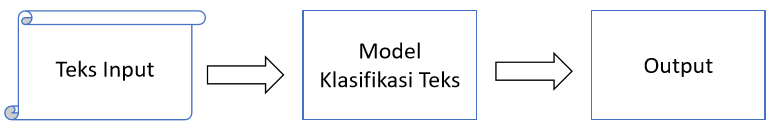
\includegraphics[width=4cm]{figures/1174062/4/Teori/No1.png}
		\caption{Gambar Klasifikasi Data}
	\end{figure}
	
\item Jelaskan mengapa klasifikasi bunga tidak bisa menggunakan machine learning, sertakan ilustrasi sendiri.

Karna Machine Learning tidak dapat menampilkan atau tidak dapat memberikan output sesuai dengan apa yang telah inputkan sebelumnya.hal ini terjadi karena mesin yang membeikan output atau yang biasa dikenal dengan noise. Contohnya dalah Ketika kita menginputkan sebuah label yang di dalamnya berupa Bungan, akan tetapi nantinya output yang di proses oleh mesin tersebut adalah labeh yang berbeda. 

	\begin{figure}[H]
	\centering
		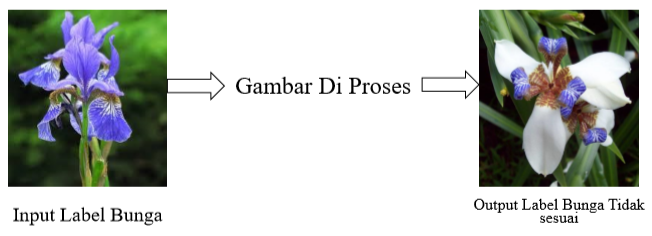
\includegraphics[width=4cm]{figures/1174062/4/Teori/No2.png}
		\caption{Gambar Proses Klasifikasi Bunga}
	\end{figure}
	
\item Jelaskan teknik pembelajaran mesin pada teks kata-kata yang digunakan di youtube, jelaskan arti per atribut data csv dan sertakan ilustrasi sendiri.

Salah satu Teknik pembelajaran yang ada di youtube adalah dengan menggunakan keyword. Seperti halnya Ketika kita mau mencari sebuah video pada youtube, kita tinggal mengetikkan sebuah keyword maka selanjutnya akan di proses untuk menampilkan hasil sesuai dengan keyword yang kita inputkan tadi. 

	\begin{figure}[H]
	\centering
		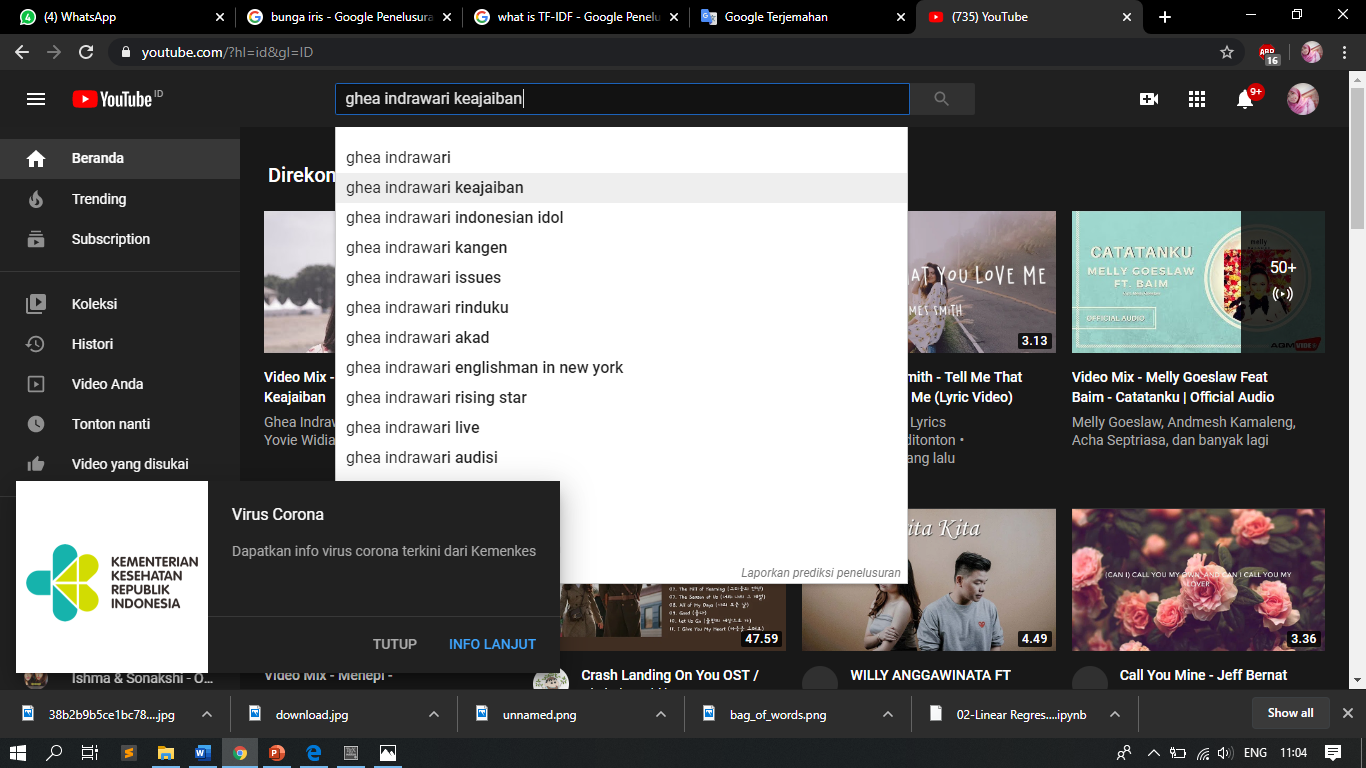
\includegraphics[width=4cm]{figures/1174062/4/Teori/No3.png}
		\caption{Gambar Machine Learning Di Youtube}
	\end{figure}

\item Jelaskan apa itu vektorisasi data.

Vektorisasi adalah sebuah proses konversi data raster menjadi sebuah vector yang umum, ini disebut dengan digitalisasi sedangkan aktifitasnya ini disebut dengan istilah digitasi. Vektorisasi adalah proses mengubah algoritma dari operasi pada nilai tunggal pada suatu waktu untuk beroperasi pada satu set nilai pada satu waktu.

\item Jelaskan apa itu Bag of Words dengan kata-kata sederhana dan ilustrasi sendiri.

BOW adalah singkatan dari Bag of Words yang merupakan sebuah metode untuk mengekstrak sebuah fitur dari dokumen teks. Fitur ini dapat kita gunakan dalam pelatihan machine learning algorithm. Fitur yang menciptakan kosakata dari semua kata yang unik disemua dokumen.

	\begin{figure}[H]
	\centering
		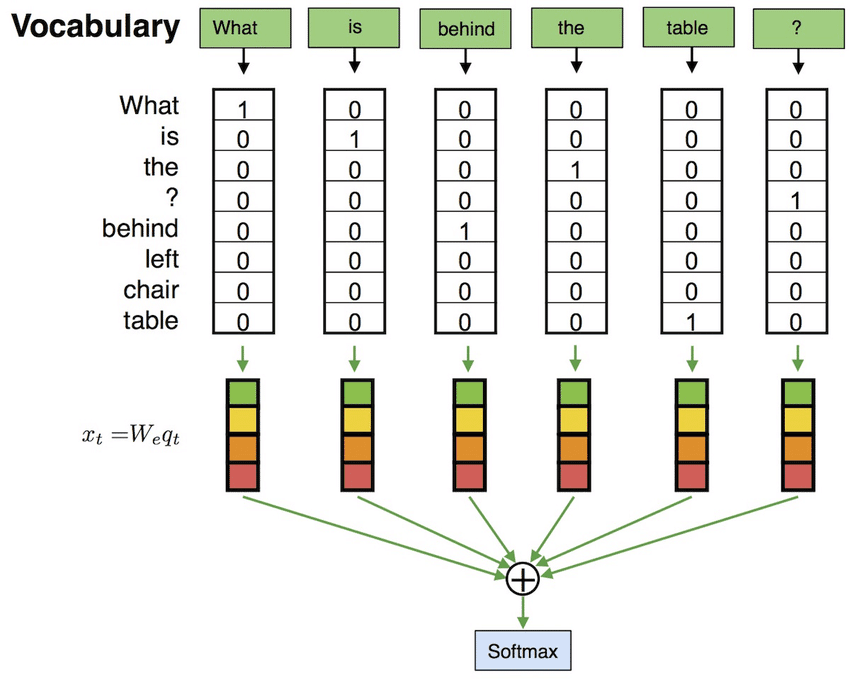
\includegraphics[width=4cm]{figures/1174062/4/Teori/No5.png}
		\caption{Gambar Rumus Bag of Words}
	\end{figure}

\item Jelaskan apa itu TF-IDF, ilustrasikan gambar sendiri.

TF-IDF adalah singkatan dari Term Frequency - Inverse Term Frequency. Bagian TF menghitung berapa kali suatu kata terjadi dalam korpus yang diberikan. Karena corpus terdiri dari banyak dokumen, setiap dokumen dan kata-katanya akan memiliki jumlah TF mereka sendiri. Bagian IDF menghitung seberapa jarang suatu kata muncul di dalam dokumen.

	\begin{figure}[H]
	\centering
		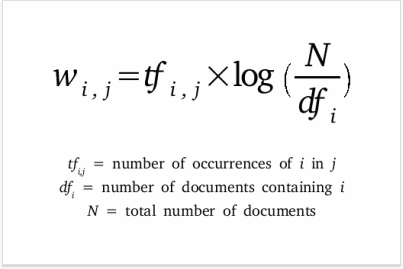
\includegraphics[width=4cm]{figures/1174062/4/Teori/No6.png}
		\caption{Gambar TF-IDF}
	\end{figure}
\end{enumerate}

\subsection{Praktek Program}
\begin{enumerate}

\item Aplikasi sederhana menggunakan pandas, membuat data dummy format csv sebanyak 500 baris dan melakukan load dataframe pandas.

	\hfill\break
	\lstinputlisting[firstline=8, lastline=12]{src/1174062/4/1174062.py}
	
	\begin{figure}[H]
	\centering
		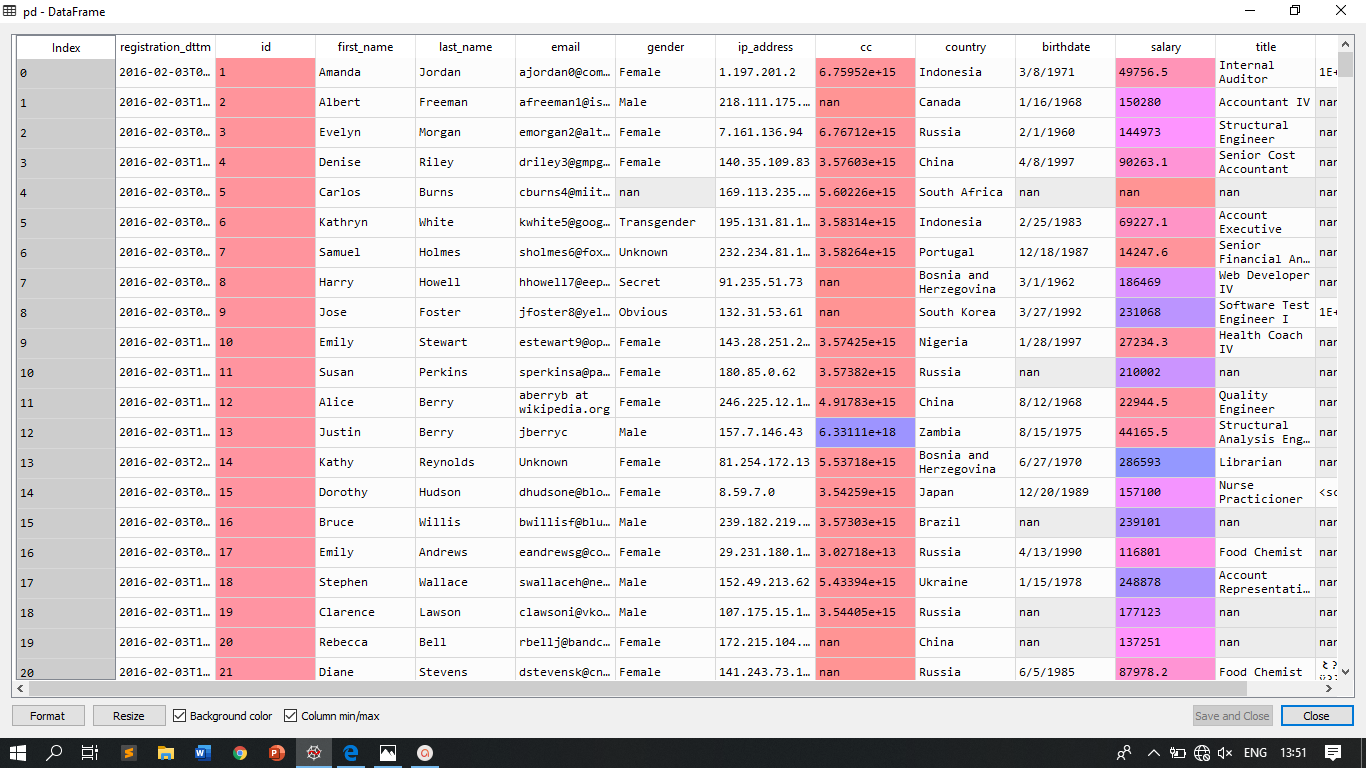
\includegraphics[width=4cm]{figures/1174062/4/Teori/1.png}
		\caption{Gambar Hasil Soal 1}
	\end{figure}

\item Dari data frame No 1 dipecah menjadi dua dataframe yaitu 450 row pertama dan 50 row sisanya.\

	\hfill\break
	\lstinputlisting[firstline=13, lastline=17]{src/1174062/4/1174062.py}

	\begin{figure}[H]
	\centering
		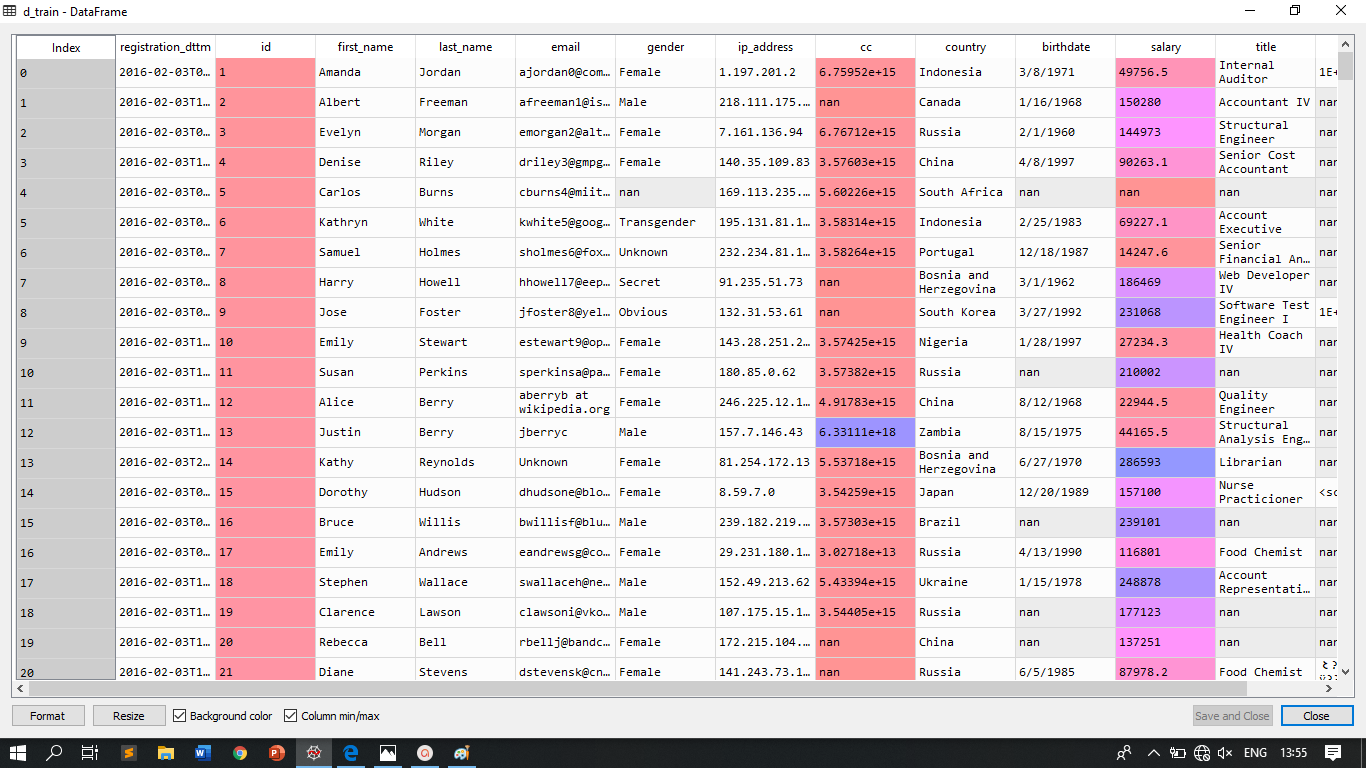
\includegraphics[width=4cm]{figures/1174062/4/Teori/2 1.png}
		\caption{Gambar Hasil 450 Row Pertama}
	\end{figure}
	
	\begin{figure}[H]
	\centering
		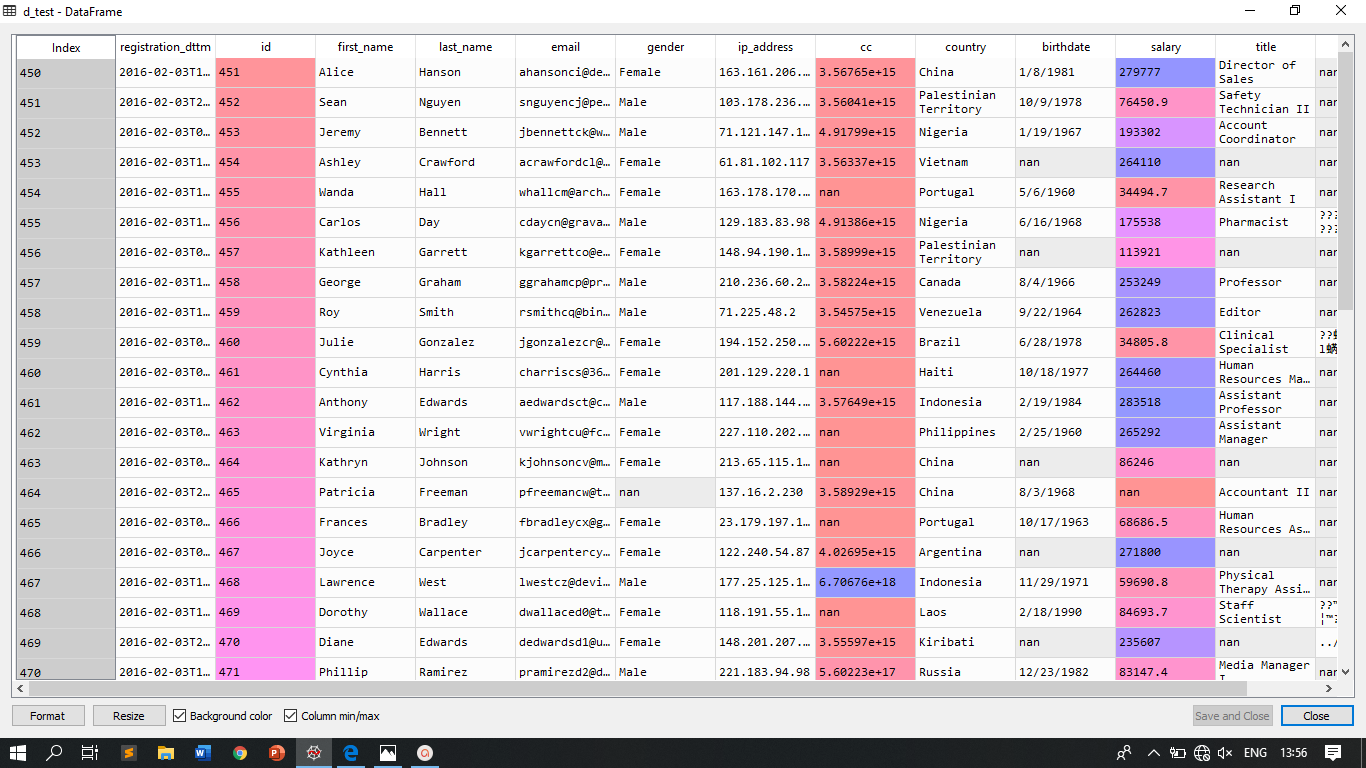
\includegraphics[width=4cm]{figures/1174062/4/Teori/2 2.png}
		\caption{Gambar Hasil 50 Row Sisanya}
	\end{figure}

\item Vektorisasi dan klasifikasi data dengan Desicion Tree.

	\hfill\break
	\lstinputlisting[firstline=18, lastline=44]{src/1174062/4/1174062.py}

	\begin{figure}[H]
	\centering
		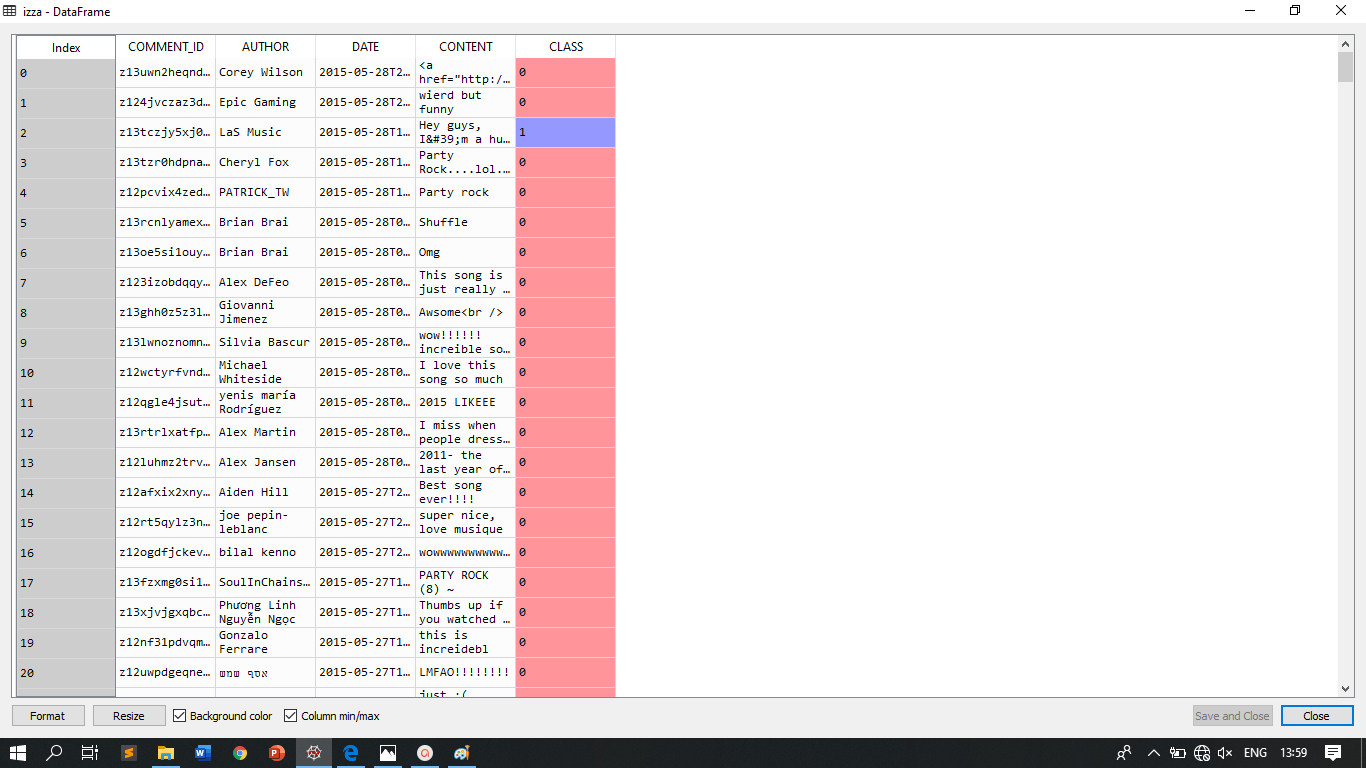
\includegraphics[width=4cm]{figures/1174062/4/Teori/3.png}
		\caption{Gambar Hasil Soal 3}
	\end{figure}

\item Mengklasifikasikan data vektorisasi dengan klasifikasi SVM.

	\hfill\break
	\lstinputlisting[firstline=45, lastline=50]{src/1174062/4/1174062.py}

	\begin{figure}[H]
	\centering
		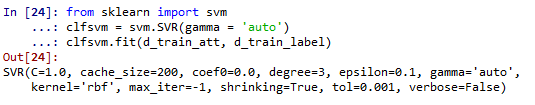
\includegraphics[width=4cm]{figures/1174062/4/Teori/4.png}
		\caption{Gambar Hasil Soal 4}
	\end{figure}

\item Mengklasifikasi data vektorisasi dengan klasifikasi Desicion tree.

	\hfill\break
	\lstinputlisting[firstline=51, lastline=56]{src/1174062/4/1174062.py}

	\begin{figure}[H]
	\centering
		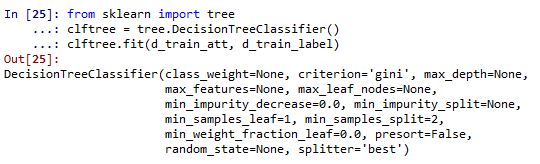
\includegraphics[width=4cm]{figures/1174062/4/Teori/5.png}
		\caption{Gambar Hasil Soal 5}
	\end{figure}
	
\item Plot confusion Matrix Menggunakan matlotlip.

	\hfill\break
	\lstinputlisting[firstline=57, lastline=79]{src/1174062/4/1174062.py}

	\begin{figure}[H]
	\centering
		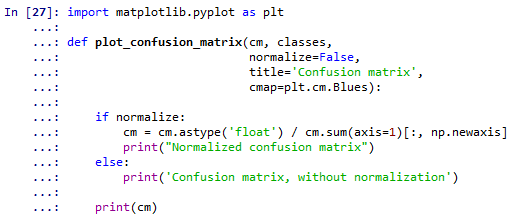
\includegraphics[width=4cm]{figures/1174062/4/Teori/6.png}
		\caption{Gambar Hasil Soal 6}
	\end{figure}
	
\item Jalankan cross validation 

	\hfill\break
	\lstinputlisting[firstline=80, lastline=88]{src/1174062/4/1174062.py}

	\begin{figure}[H]
	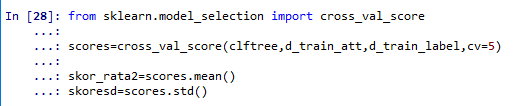
\includegraphics[width=4cm]{figures/1174062/4/Teori/7.png}
	\centering
	\caption{Gambar Hasil Soal Nomor 7}
	\end{figure}

\item Membuat program pengamatan komponen informasi .

	\hfill\break
	\lstinputlisting[firstline=89, lastline=105]{src/1174062/4/1174062.py}
\end{enumerate}

\subsection{Penanganan Error}
\begin{enumerate}
\item Dengan menyesuaikan letak file csv pada codingannya, sehingga dapat  di baca atau dipanggil file csvnya.

	\begin{figure}[H]
	\centering
		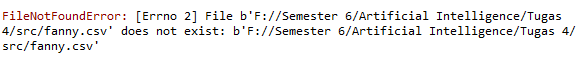
\includegraphics[width=4cm]{figures/1174062/4/Error/1.png}
		\caption{Gambar Error}
	\end{figure}
\end{enumerate}

\subsection{Bukti Tidak Plagiat}
\begin{enumerate}
\item Berikut adalah gambar bukti tidak melakukan Plagiat

\begin{figure}[H]
	\centering
		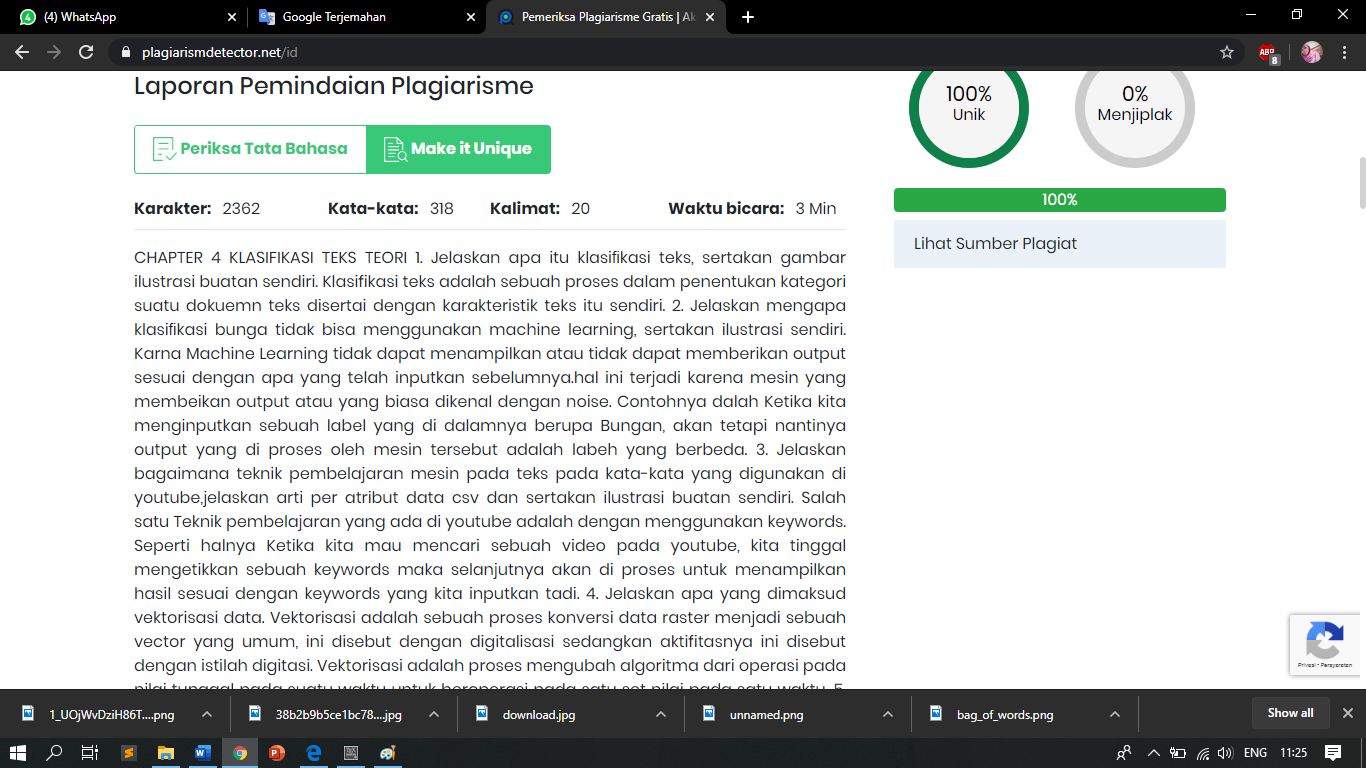
\includegraphics[width=4cm]{figures/1174062/4/Plagiat/tidakplagiat.png}
		\caption{Gambar Bukti Tidak Plagiat}
	\end{figure}
\end{enumerate}

\subsection{Link Youtube}
\begin{enumerate}
\item Berikut adalah lampiran Link Youtube untuk Chapter 4

https://www.youtube.com/watch?v=zX3W99EB2ks
\end{enumerate}